%%%%%%%%%%%%%%%%%%%%%%%%%%%%%%%%%%%%%%%%%%%%%%%%%%%%%%%%%%%%%%%%%%%%%%%%%%%%%%
% Appendix A — Machine Learning Primer
%
% This appendix introduces the principal machine learning concepts used in
% this study. It is intended for readers from educational research
% backgrounds who may be less familiar with modern predictive modelling and
% reproducible computational workflows.
%
% Contents
% --------
% A.1 Why Use Machine Learning in Educational Research?
% A.2 Decision Trees and Random Forests
% A.3 Feature Importance
% • Impurity Reduction
% • Why Feature Importances Sum to Approximately One
% • Averaging Feature Importance Across Models
% A.4 ROC Curves and Model Evaluation
% A.5 Hyperparameter Tuning
% A.6 Prediction and Explanation: Why Statistical Models and Machine Learning
% Were Both Used
% A.7 Reproducible Computational Workflows
%%%%%%%%%%%%%%%%%%%%%%%%%%%%%%%%%%%%%%%%%%%%%%%%%%%%%%%%%%%%%%%%%%%%%%%%%%%%%%
%%%%%%%%%%%%%%%%%%%%%%%%%%%%%%%%%%%%%%%%%%%%%%%%%%%%%%%%%%%%%%%%%%%%%%%%%%%%%%
% Planned Figures
%
% Figure A.1  Simple Decision Tree (planned)
% Figure A.2  Random Forest Concept (planned)
% Figure A.3  Individual Feature Importance (generated)
% Figure A.4  Grouped Feature Importance (generated)
% Figure A.5  ROC Comparison (generated)
% Figure A.6  Reproducible Computational Workflow (planned)
%
% (Insert only where they improve understanding.)
%%%%%%%%%%%%%%%%%%%%%%%%%%%%%%%%%%%%%%%%%%%%%%%%%%%%%%%%%%%%%%%%%%%%%%%%%%%%%%

\appendix

\section{A Brief Primer on Interpretable Machine Learning for Educational Research}

This appendix provides a concise introduction to the principal machine learning concepts used throughout this study. It is intended for readers with a background in 
educational research who may be less familiar with predictive modelling. The appendix is explanatory rather than comprehensive and is designed to support interpretation 
of the methods and results presented in the main paper.


\subsection*{Part I — Machine Learning Foundations}
\subsection{Why Use Machine Learning in Educational Research?}

Educational researchers have traditionally used statistical models to examine relationships between variables and explain differences in student outcomes. 
Machine learning complements these approaches by placing greater emphasis on prediction. Rather than beginning with a small set of predefined relationships, 
machine learning models can identify patterns across many variables and evaluate how well those patterns generalise to new data.

In educational settings, this can be useful when the research aim is not only to explain why students succeed or struggle, but also to identify which 
combinations of prior preparation, academic history, and student characteristics are most informative. When used carefully, machine learning can therefore 
support early identification, model comparison, and evidence-informed intervention without replacing the need for educational interpretation.

\subsection{Prediction and Explanation}

Statistical modelling and machine learning often overlap, but they usually emphasise different questions. Statistical models commonly focus on estimating relationships, 
testing hypotheses, and explaining how particular variables are associated with an outcome. Machine learning models place greater emphasis on predictive performance: how 
accurately a model can classify or estimate outcomes for observations that were not used during model fitting.

Neither emphasis is inherently superior. The appropriate approach depends on the research question. In educational research, explanation is essential when the aim is to 
understand mechanisms, evaluate theory, or estimate the effect of an intervention. Prediction is valuable when the aim is to identify students who may require support, 
compare alternative models, or detect complex patterns that may not be captured by a simpler predefined relationship. Used together, statistical and machine learning 
approaches can provide complementary evidence.
\subsection*{Part II — Tree-Based Machine Learning}
\subsection{Decision Trees}

A decision tree is one of the simplest and most interpretable machine learning models. It predicts an outcome by repeatedly dividing the data into smaller groups 
according to decision rules based on the available predictor variables. Each split is chosen to maximise the separation between observations with different outcomes, 
producing a tree-like structure that can be followed from the root node to a final prediction. Figure~\ref{fig:decision_tree_primer} illustrates the basic structure of a 
decision tree, showing how successive decision rules partition observations into increasingly homogeneous groups.

One of the principal advantages of decision trees is their transparency. Every prediction can be traced through a sequence of explicit decisions, allowing researchers to 
understand why a particular outcome was reached. For this reason, decision trees are widely used as both predictive models and explanatory tools, particularly in educational 
research where interpretability is often as important as predictive accuracy.

\begin{figure}[ht]
\centering
% TODO: Insert Figure A.1 — Simple Decision Tree
\fbox{\parbox{0.8\textwidth}{\centering
Figure A.1 Placeholder\\
Simple conceptual decision tree}}
\caption{A simplified decision tree illustrating how successive decision rules partition observations into increasingly homogeneous groups.}
\label{fig:decision_tree_primer}
\end{figure}

\subsection{Random Forests}

Although decision trees are easy to interpret, they can be sensitive to small changes in the training data. A different sample of observations may produce a noticeably 
different tree, reducing the stability of predictions. Random forests address this limitation by combining the predictions of many decision trees rather than relying on a 
single model.

Each tree in a random forest is trained using a different bootstrap sample of the available data, and at each decision point only a random subset of predictor variables is 
considered. This deliberate introduction of randomness produces a diverse collection of trees whose combined prediction is typically more accurate and more robust than that 
of an individual tree. The final prediction is obtained by aggregating the predictions from all trees, commonly through majority voting for classification problems or 
averaging for regression problems. The overall concept is illustrated in Figure~\ref{fig:random_forest_primer}, where the predictions of multiple decision trees are 
aggregated to produce a single, more stable prediction.

\begin{figure}[ht]
\centering
% TODO: Insert Figure A.2 — Random Forest Concept
\fbox{\parbox{0.8\textwidth}{\centering
Figure A.2 Placeholder\\
Random Forest Concept}}
\caption{A conceptual illustration showing how multiple decision trees are combined to produce a single prediction.}
\label{fig:random_forest_primer}
\end{figure}

Random forests generally achieve higher predictive performance than individual decision trees while still providing valuable information about the relative importance of 
predictor variables. For this reason, they have become one of the most widely used interpretable machine learning methods in educational data analysis.

\subsection{Feature Importance}

Many machine learning models can provide more than accurate predictions; they can also indicate which variables contributed most strongly to those predictions. 
This measure is commonly referred to as \emph{feature importance}. In tree-based models, feature importance reflects the extent to which each predictor contributes to 
reducing classification error across all decision trees in the model. The individual predictor importances obtained in this study are shown in 
Figure~\ref{fig:feature_importance_individual}, illustrating the relative contribution of each predictor to the tuned tree-based models.

\begin{figure}[ht]
\centering
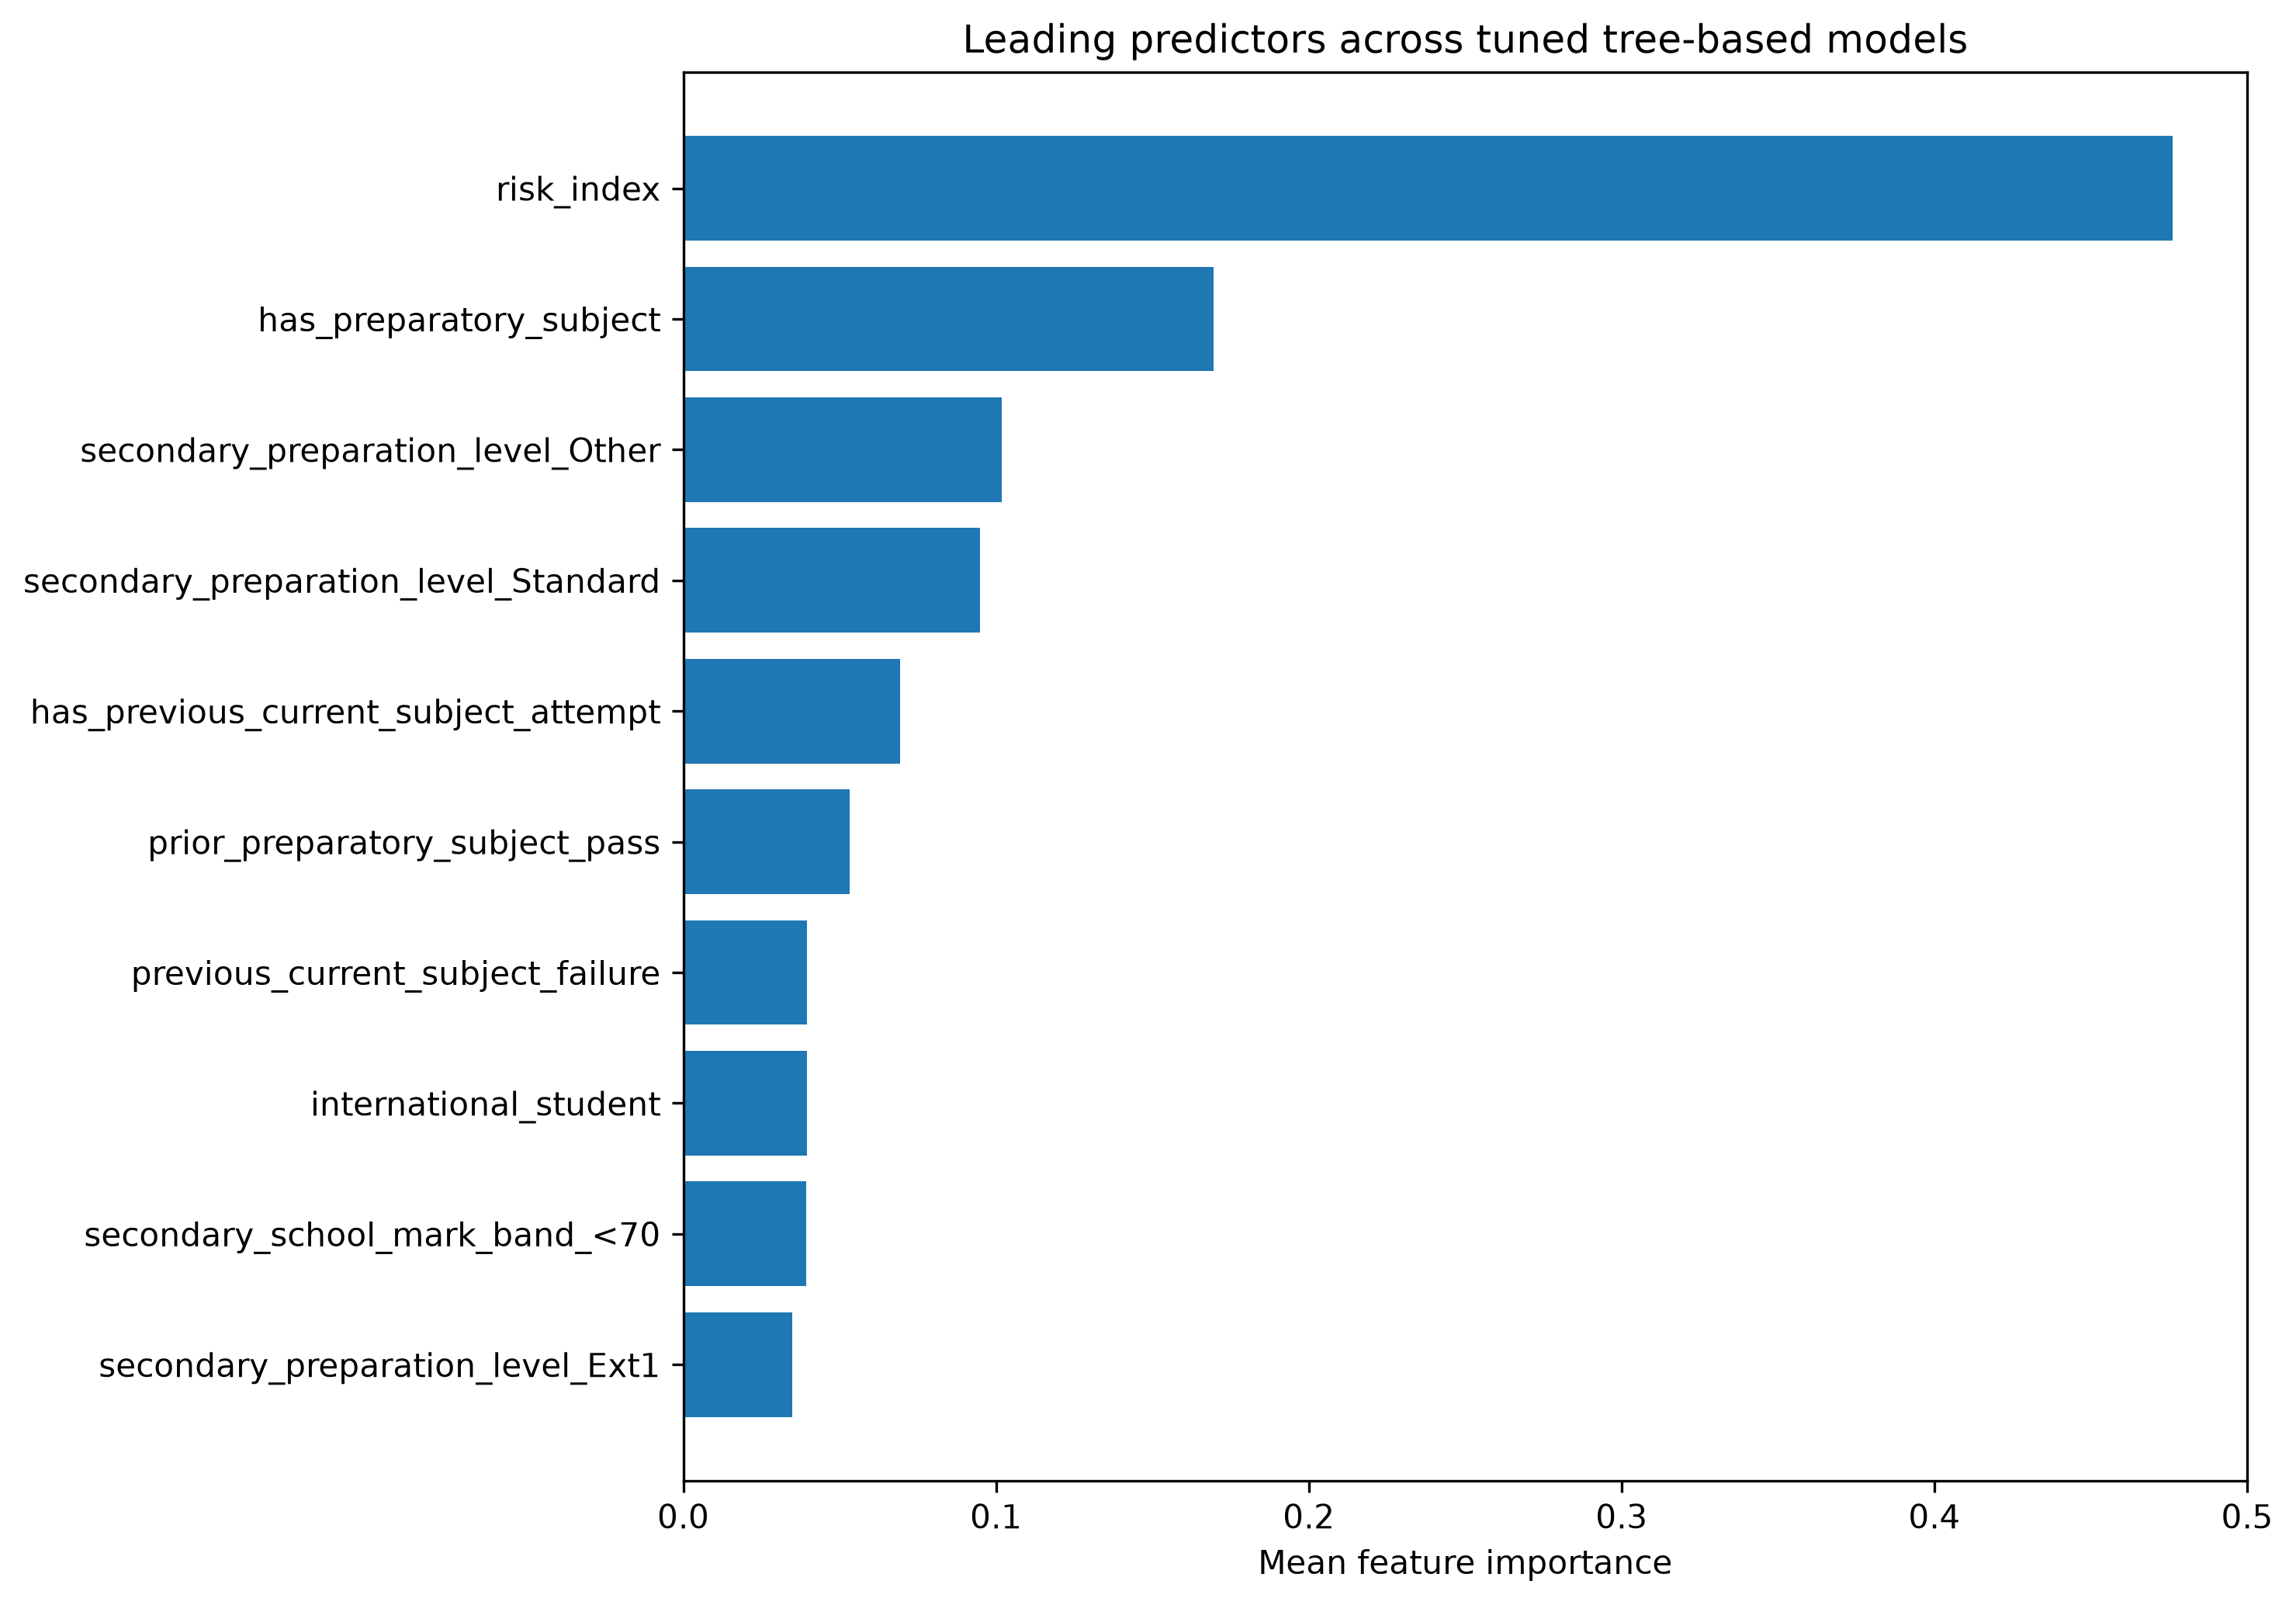
\includegraphics[
    width=\textwidth
]{../figures/fig_tuned_feature_importance_individual.png}
\caption{Individual feature importance values produced by the tuned tree-based models. Variables with larger importance contributed more strongly to the model's predictions.}
\label{fig:feature_importance_individual}
\end{figure}

Feature importance should be interpreted as a relative measure rather than an absolute effect size. The values indicate the comparative contribution of each predictor 
within a particular model and typically sum to one. Consequently, a feature with an importance of 0.30 contributed approximately twice as much to the model's predictive 
decisions as a feature with an importance of 0.15, but this does not imply a causal relationship.

In this study, feature importance was examined at two levels. Individual predictor variables were first evaluated within each model. Related variables were then 
aggregated into broader educational themes, including secondary mathematics preparation, previous university performance, preparatory mathematics, secondary school 
achievement, student characteristics, and the composite risk measure. This grouped interpretation provides a clearer educational perspective while preserving the 
underlying machine learning results.


\subsection{Grouped Feature Importance}

Individual feature importance values provide detailed information about the contribution of specific predictor variables. However, educational researchers are often 
interested in broader concepts rather than individual dummy-coded variables. For example, several variables may represent different levels of secondary mathematics 
preparation, while others describe previous university performance or participation in preparatory mathematics subjects.

To improve interpretability, this study grouped related predictor variables into educational themes before calculating their combined importance. This approach 
preserves the predictive information produced by the machine learning models while presenting the results in a form that is more closely aligned with educational theory 
and practice. Rather than interpreting numerous individual variables, readers can evaluate the relative importance of broader constructs that are meaningful within the 
context of student transition. The resulting grouped feature importance values are presented in Figure~\ref{fig:feature_importance_grouped}, providing an educational 
interpretation of the model outputs by aggregating related predictors into broader conceptual themes.

\begin{figure}[ht]
\centering
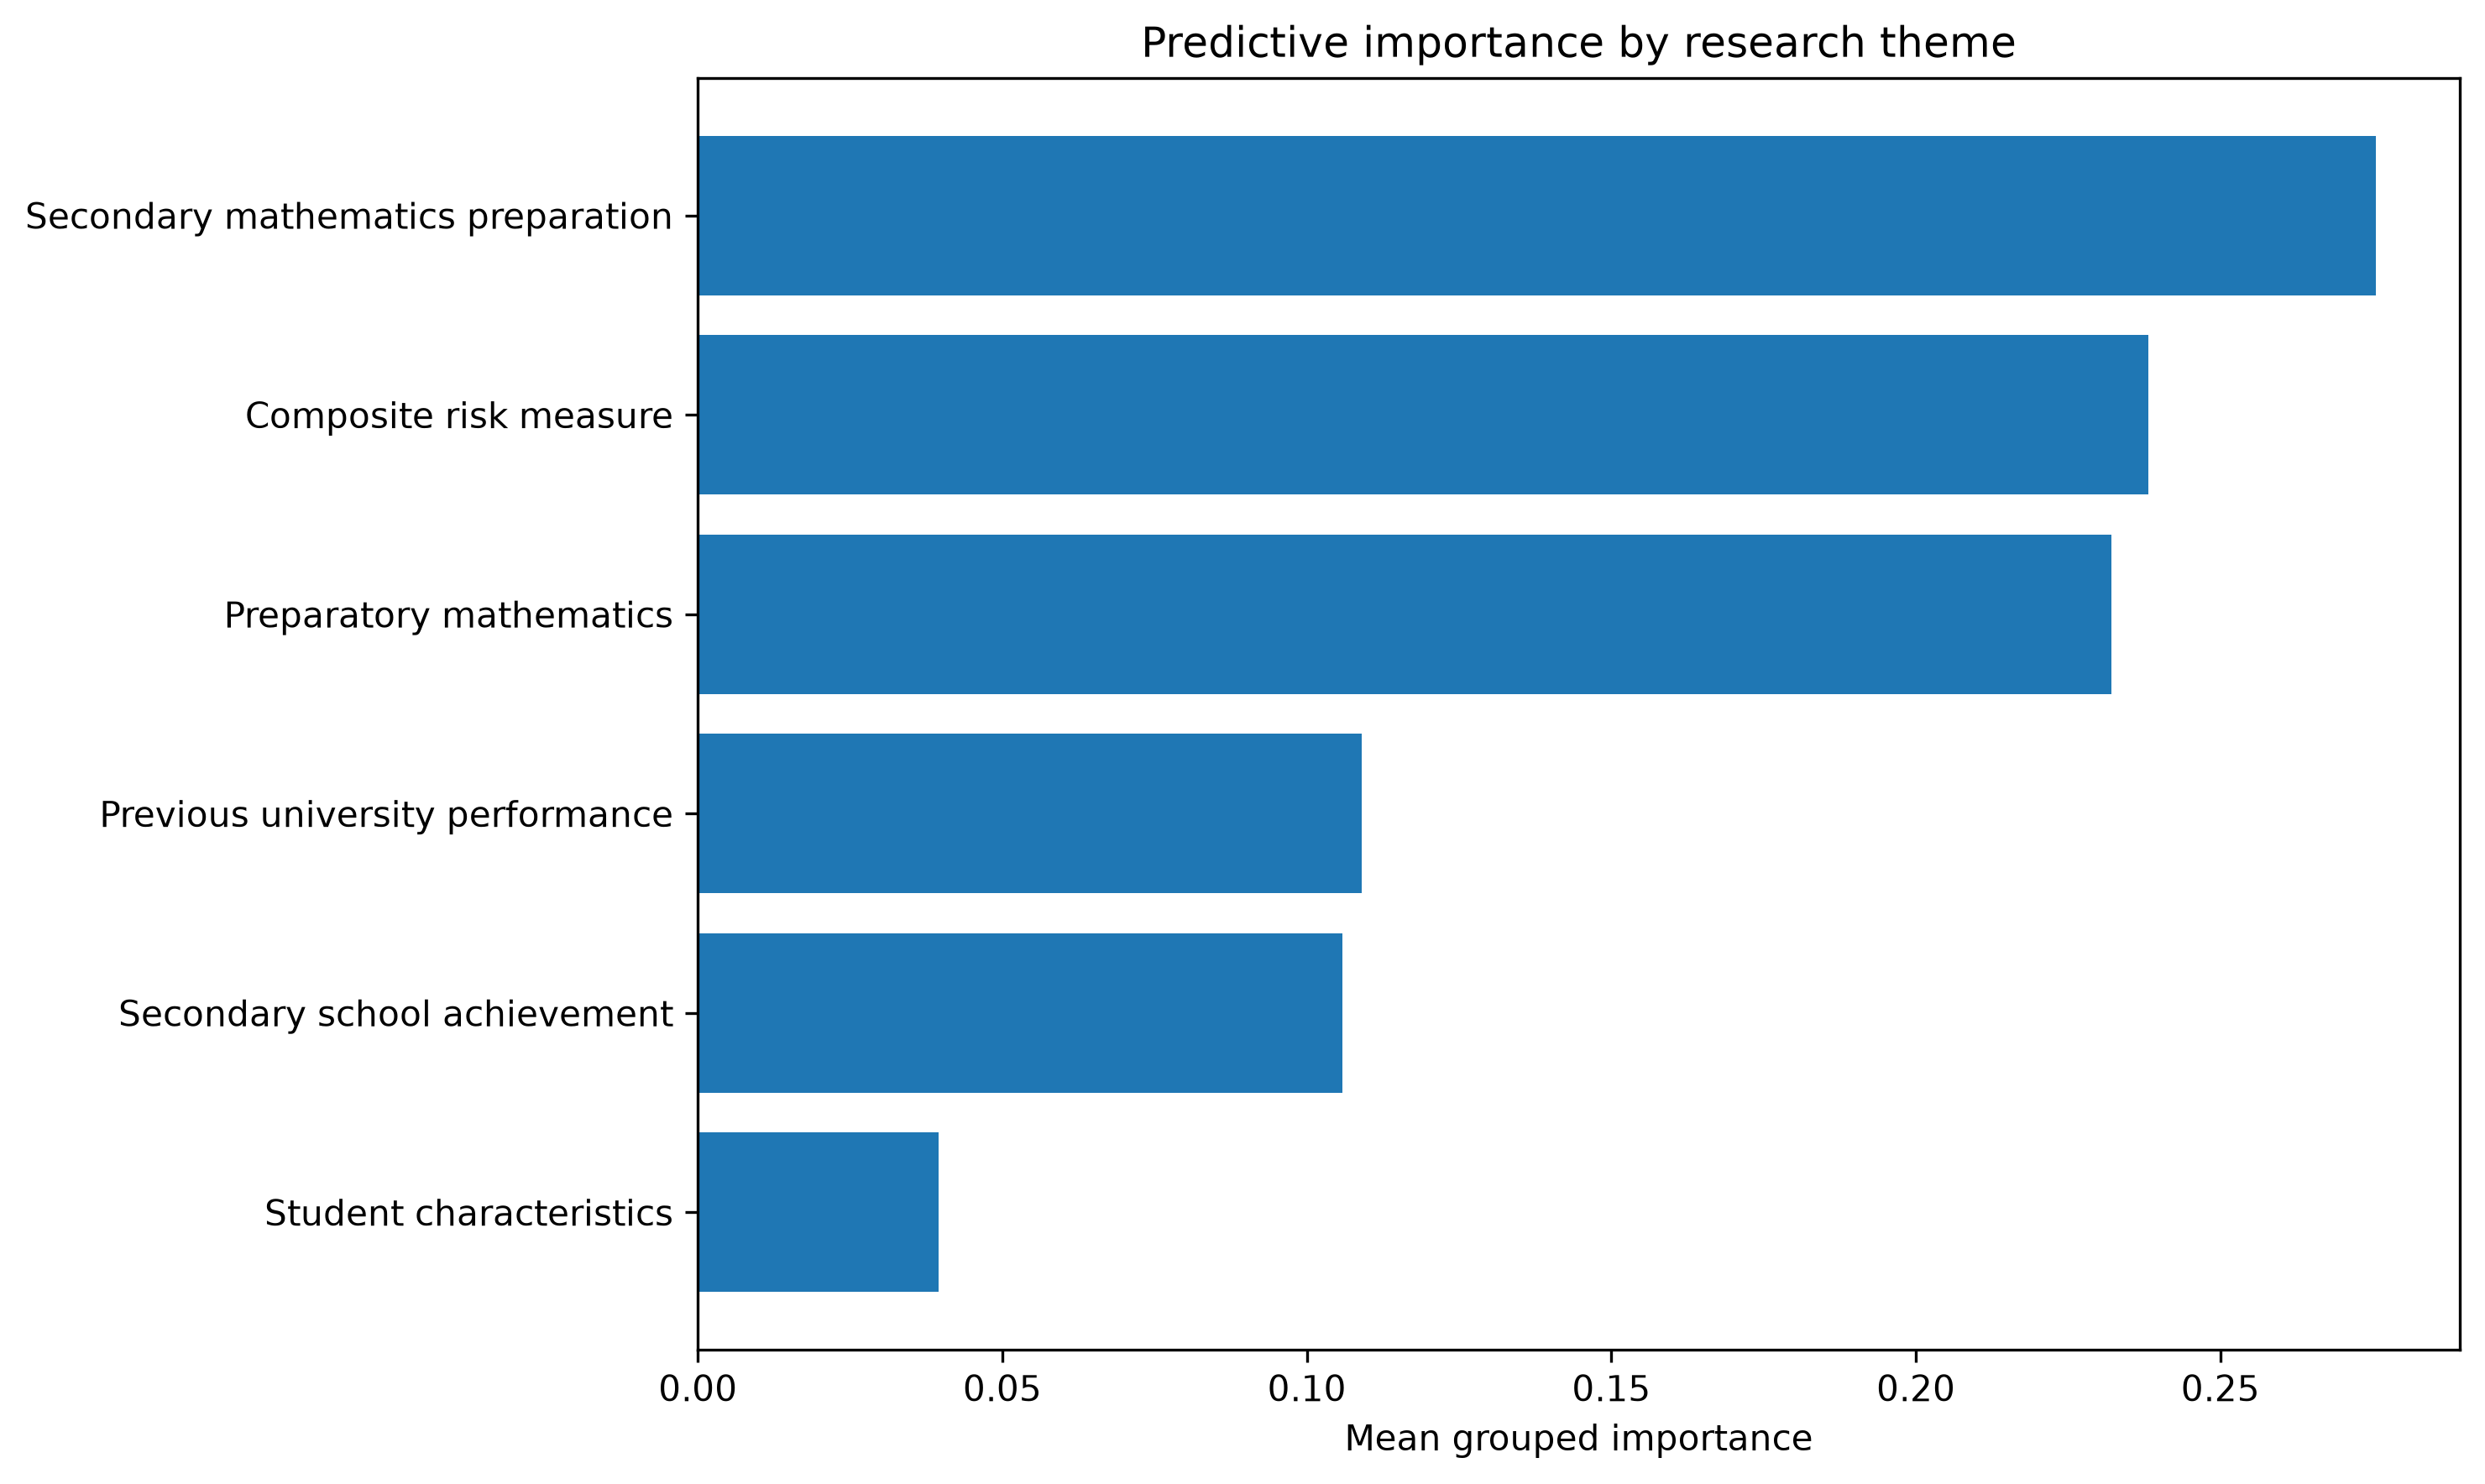
\includegraphics[
    width=\textwidth
]{../figures/fig_tuned_feature_importance_grouped.png}
\caption{Grouped feature importance values showing the relative contribution of broader educational themes across the tuned tree-based models.}
\label{fig:feature_importance_grouped}
\end{figure}

Grouping feature importance therefore provides an additional interpretative layer. It bridges the gap between machine learning outputs and educational understanding by 
translating technical model results into concepts that can be discussed within the broader literature on student preparation, transition, and academic success.

\subsection*{Part III — Model Development and Evaluation}
\subsection{Training and Test Data}

A fundamental principle of machine learning is that model performance should be evaluated using data that were not used during model training. If a model is assessed 
only on the observations from which it learned, the reported performance is likely to be overly optimistic because the model has already seen those examples.

To address this issue, the available data are commonly divided into two subsets. The training dataset is used to construct and tune the model, while the test dataset is 
reserved for an independent evaluation of predictive performance. The test data therefore provide a more realistic indication of how well the model is expected to perform 
when applied to new students.

This study adopted a reproducible train--test split, ensuring that all candidate models were evaluated using the same independent test dataset. This approach provides a 
fair comparison between models and reduces the likelihood that reported performance reflects random variation in the training data rather than genuine predictive capability.


\subsection{Cross-Validation}

A single train--test split provides one estimate of model performance, but the result may depend on the particular observations assigned to each subset. 
Cross-validation reduces this dependence by repeatedly dividing the training data into different partitions and evaluating the model across multiple iterations.

In (k)-fold cross-validation, the training data are divided into (k) approximately equal subsets. During each iteration, one subset is reserved for validation 
while the remaining subsets are used for model training. This process is repeated until every subset has served as the validation set exactly once. 
The resulting performance measures are then averaged to provide a more stable estimate of model performance.

Cross-validation is particularly valuable during model development because it helps identify models that generalise well rather than those that perform well 
only for a particular sample of training data. For this reason, it is commonly used during hyperparameter tuning before a final evaluation is performed on the 
independent test dataset.

\subsection{Hyperparameter Tuning}

Many machine learning models include settings, known as hyperparameters, that influence how the model is constructed. For example, a decision tree may be limited by its 
maximum depth, while a random forest requires the number of trees to be specified before training begins. These values are chosen by the researcher rather than learned 
directly from the data.

Hyperparameter tuning is the process of systematically evaluating different combinations of these settings to identify those that produce the best predictive performance. 
This evaluation is commonly performed using cross-validation so that each candidate configuration is assessed consistently across multiple training and validation partitions.

Careful hyperparameter tuning improves model robustness and reduces the risk of selecting a model that performs well only because of a particular choice of settings. 
In this study, all candidate models were tuned before their final performance was evaluated on the independent test dataset, ensuring that comparisons were both fair and 
reproducible.


\subsection{ROC Curves and Model Evaluation}

Receiver Operating Characteristic (ROC) curves provide a standard method for evaluating the discriminatory performance of binary classification models. Rather than 
assessing a model using a single classification threshold, an ROC curve summarises performance across all possible thresholds by plotting the true positive rate (sensitivity) 
against the false positive rate (1 -- specificity). This provides a threshold-independent assessment of how effectively a model distinguishes between the two outcome classes.

The overall discriminatory ability of a model is commonly summarised by the Area Under the ROC Curve (AUC). An AUC value of 0.5 indicates performance equivalent to random 
guessing, whereas a value of 1.0 represents perfect discrimination. In educational prediction studies, the ROC curve therefore provides a useful complement to measures such 
as accuracy, precision, and recall because it evaluates the model's ability to rank students according to their likelihood of success or failure, independent of any particular 
decision threshold. The ROC curves for the tuned decision tree and random forest models are presented in Figure~\ref{fig:roc_curve_primer}, allowing their discriminatory 
performance to be compared across all classification thresholds.

In this study, ROC curves were used to compare the predictive performance of the tuned decision tree and random forest models using the independent test dataset. This approach 
enabled the relative discriminatory performance of the competing models to be evaluated consistently and provided an objective basis for selecting the best-performing model 
while reducing the influence of any single classification threshold.

\begin{figure}[ht]
\centering
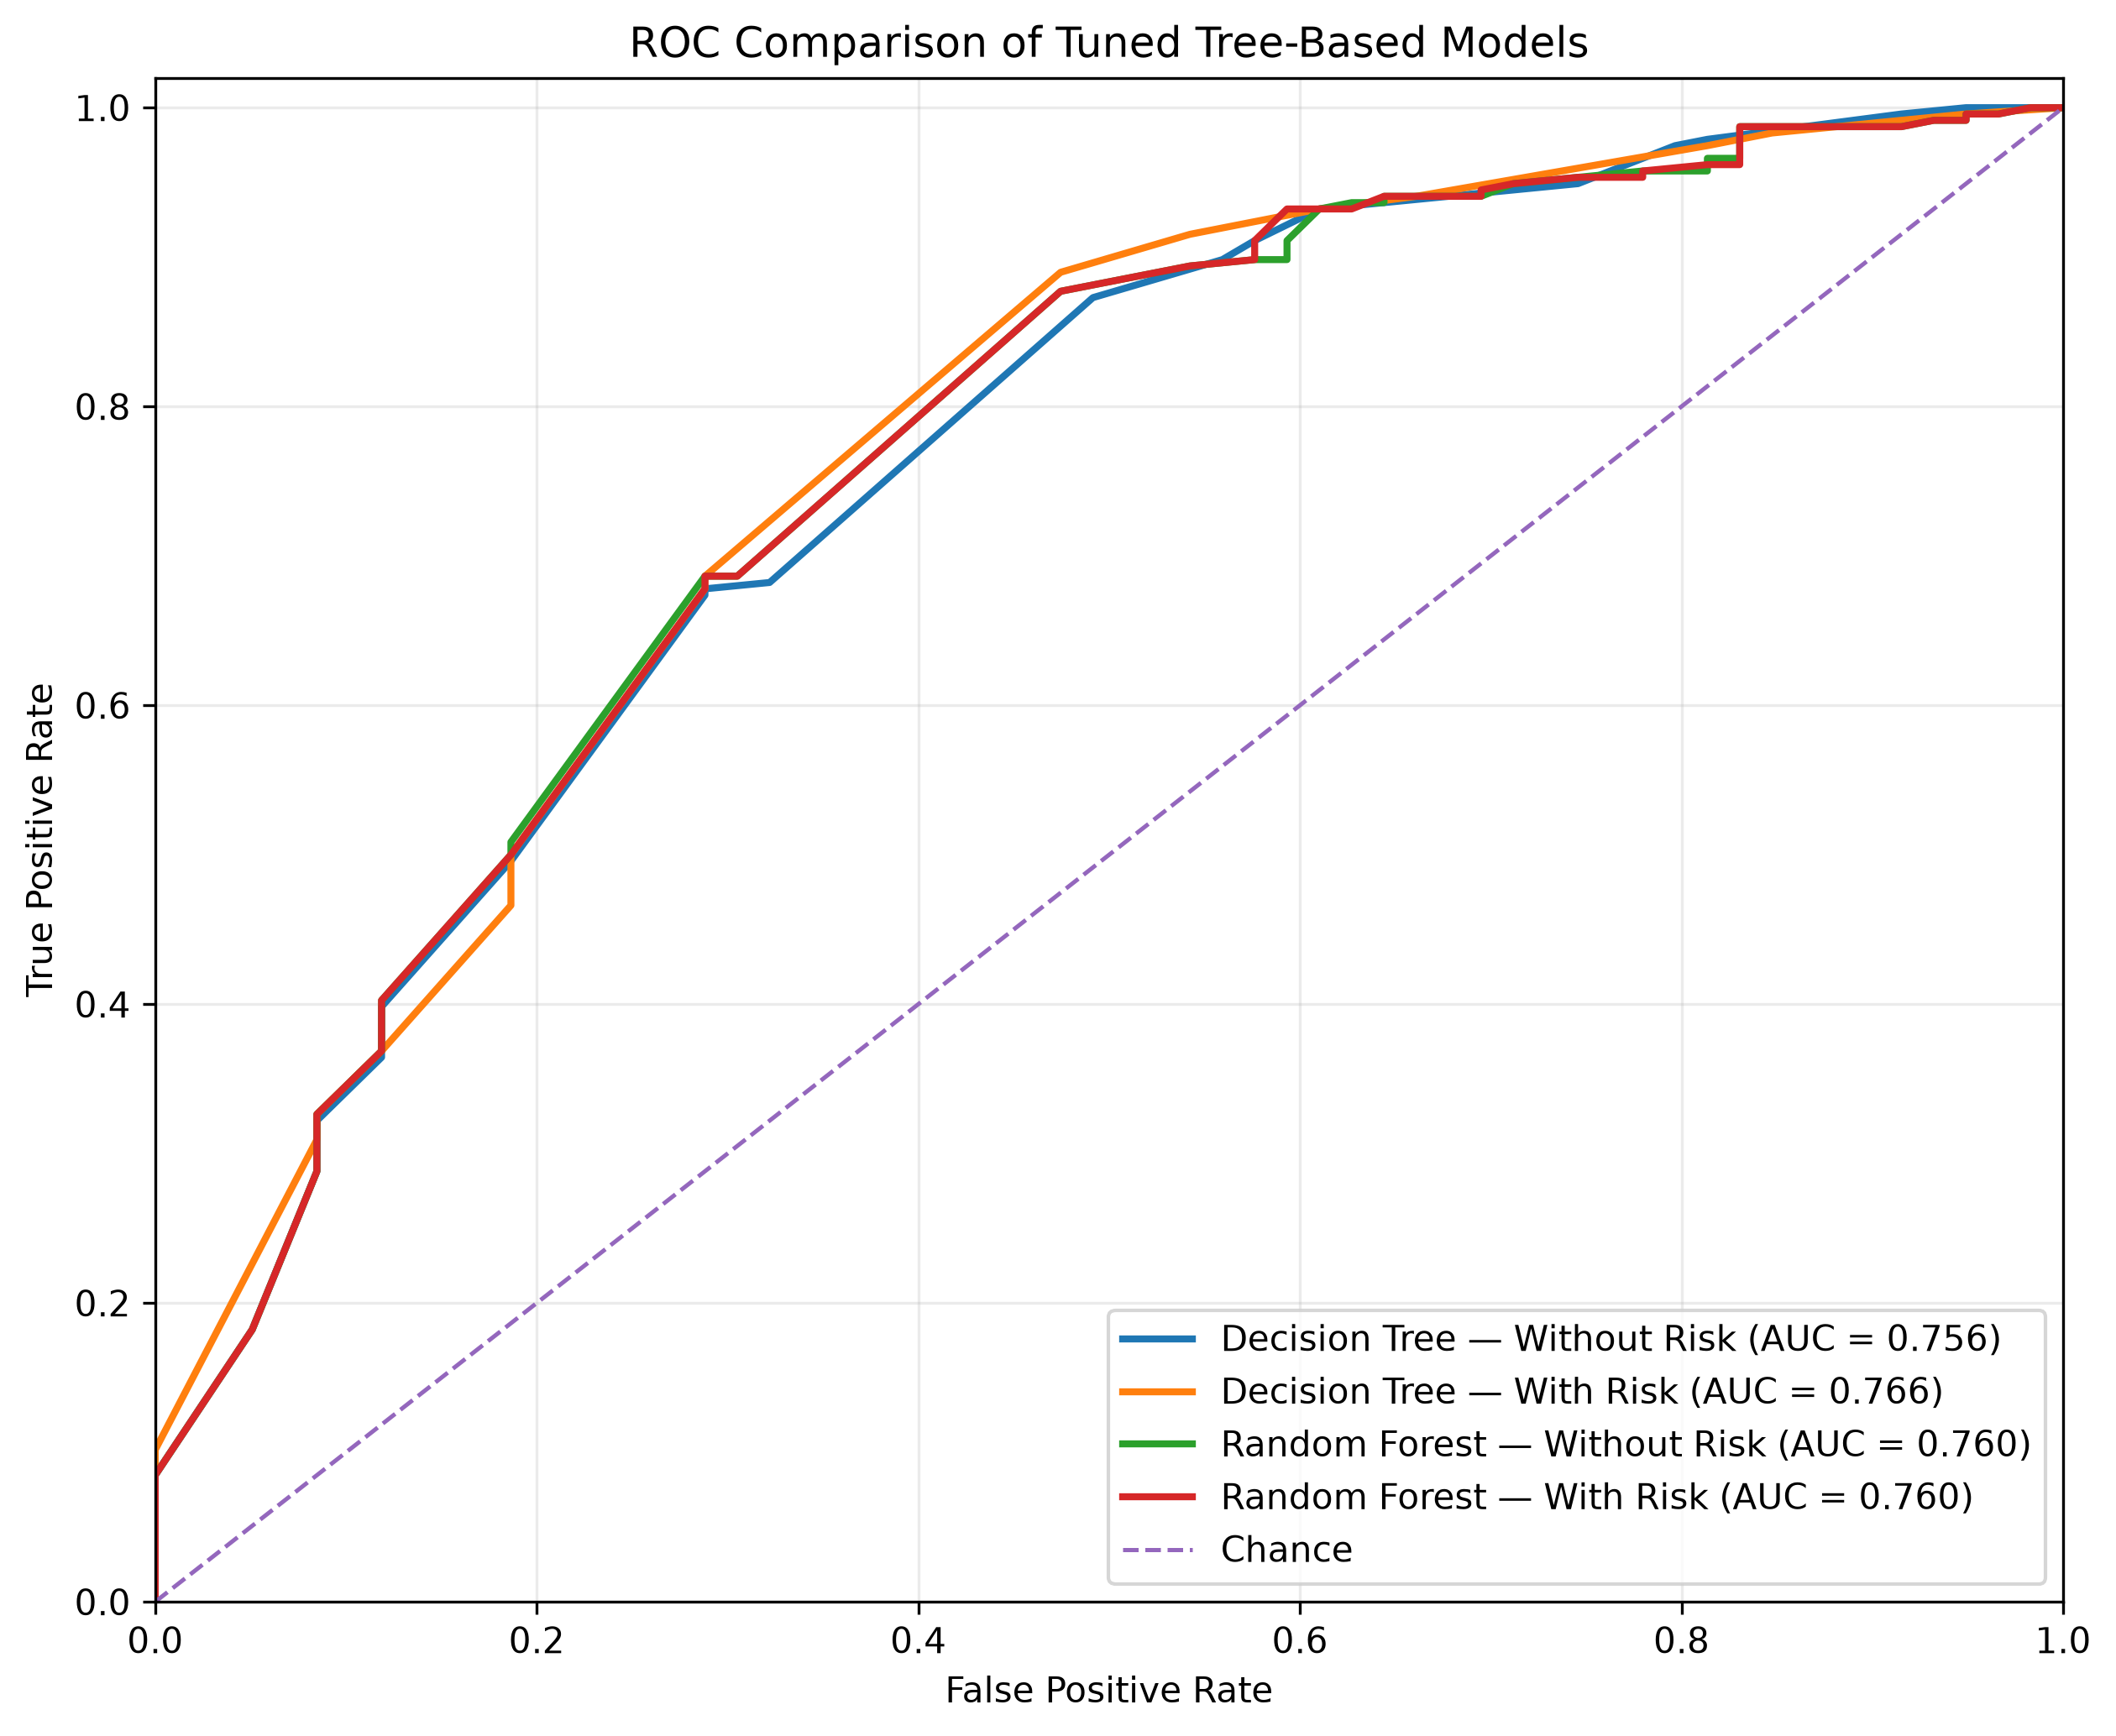
\includegraphics[width=0.75\textwidth]{../figures/fig_tuned_tree_roc_comparison.png}
\caption{Receiver Operating Characteristic (ROC) curves comparing the discrimination performance of the tuned tree-based models on the independent test dataset. Curves closer to the upper-left corner indicate stronger discriminatory performance, while the area under each curve (AUC) summarises overall model effectiveness across all classification thresholds.}
\label{fig:roc_curve_primer}
\end{figure}

\newpage

\subsection*{Part IV — Research Methodology}
\subsection{Why Statistical Models and Machine Learning Were Both Used}

Statistical modelling and machine learning provide complementary perspectives rather than competing methodologies. Statistical models are particularly valuable when the 
objective is to estimate relationships between variables, test hypotheses, and quantify uncertainty. Machine learning methods are designed to maximise predictive 
performance and to identify complex patterns that may not be apparent using traditional statistical techniques alone.

This study deliberately combined both approaches. Logistic regression provided a well-established statistical benchmark against which the machine learning models could be 
compared. Decision trees and random forests were then used to investigate predictive performance and to examine the relative importance of educational factors influencing 
student success.

Using both approaches strengthened the overall analysis. Agreement between the statistical and machine learning results increased confidence in the findings, 
while differences between the models provided additional insight into the strengths and limitations of each analytical approach.



\subsection{Reproducible Computational Workflows}

Reproducibility is a fundamental principle of modern computational research. A reproducible workflow ensures that the complete analysis, from data preparation to the 
final manuscript, can be repeated using the same source data and documented procedures. This reduces the likelihood of transcription errors, improves transparency, and 
enables other researchers to verify and extend the reported findings.

In this study, reproducibility was supported through an integrated computational workflow. Data preparation, statistical modelling, machine learning analyses, independent 
verification, figure generation, table production, and manuscript components were all produced automatically from the underlying analysis. The paper itself incorporated 
generated values directly from the analysis pipeline, ensuring consistency between reported results and computational outputs. The overall computational workflow 
developed for this research is summarised in Figure~\ref{fig:workflow_primer}, illustrating how the study progresses from raw research data through automated analysis, 
independent verification, and manuscript generation.

Such workflows provide benefits beyond a single study. They simplify maintenance, facilitate future analyses on new datasets, and support transparent, evidence-based 
educational research by ensuring that published results remain directly traceable to the underlying computations.

\begin{figure}[ht]
\centering
% TODO: Replace with workflow diagram
\fbox{\parbox{0.9\textwidth}{\centering
Figure A.6 Placeholder\\[1ex]
Reproducible Computational Workflow\\[2ex]

Raw Research Data\\
$\downarrow$\\
Data Preparation\\
$\downarrow$\\
Statistical Analysis\\
$\downarrow$\\
Machine Learning \hspace{2cm} Independent R Verification\\
\hspace{2.8cm}$\backslash$ \hspace{0.2cm}/\\
\hspace{2.9cm}$\downarrow$\\
Tables • Figures • Generated LaTeX Values\\
$\downarrow$\\
Automated Paper Generation\\
$\downarrow$\\
Publication-ready PDF}}
\caption{Overview of the reproducible computational workflow developed for this study, illustrating the progression from raw research data through analysis, independent verification, automated reporting, and final manuscript generation.}
\label{fig:workflow_primer}
\end{figure}